\documentclass[../notes.tex]{subfiles}

\pagestyle{main}
\renewcommand{\chaptermark}[1]{\markboth{\chaptername\ \thechapter\ (#1)}{}}
\setcounter{chapter}{7}

\begin{document}




\chapter{???}
\section{Specht Modules are Irreducible and Well-Defined}
\begin{itemize}
    \item \marginnote{11/13:}Announcements.
    \begin{itemize}
        \item This week's homework is the next to last one.
    \end{itemize}
    \item Review.
    \begin{itemize}
        \item Miracuously, we can understand all representations of $S_n$.
        \item We start with partitions $\lambda$ that are defined a certain way. We visualize them with Young diagrams.
        \item The number of partitions of $n$ is equal to the number of conjugacy classes in $S_n$ is equal to the number of irreps in $S_n$.
        \begin{itemize}
            \item It is a special feature of $S_n$ that this is true.
        \end{itemize}
        \item How do we construct the irreducible representation $V_\lambda$ due to $\lambda$?
        \begin{itemize}
            \item Consider $(4,2,1)'=(3,2,1,1)$ as an example (recall the definition of an inverse partition).
            \item Take Vandermonde determinants (recall the explicit definition of these, too).
            \item Then we define $V_\lambda=\C[S_n]$, take Vandermonde determinant of variables corresponding to the first column, so that $\Delta(x_1,\dots,x_{\lambda_1'})\Delta(x_{\lambda_1'+1},\dots,x_{\lambda_2'})\cdots\Delta(x_{\lambda_{k-1}'+1},\dots,\lambda_k')$.
            \item Thus, we let $\C[S_n]$ act on $(x_1-x_2)(x_1-x_3)(x_2-x_3)(x_4-x_5)$.
        \end{itemize}
    \end{itemize}
    \item One more example.
    \begin{itemize}
        \item $\lambda=(2,2)$.
        \item Let $\C[S_4]$ act on $(x_1-x_2)(x_3-x_4)$.
        \item Then
        \begin{equation*}
            V_\lambda = \inp{(x_1-x_2)(x_3-x_4),(x_1-x_3)(x_2-x_4),(x_1-x_4)(x_2-x_3)}
        \end{equation*}
        \item But we're expecting a 2D representation. Indeed, we get one because if we define the first term above to be $a$ and the second to be $b$, then the third is $b-a$. Thus, there are only two linearly independent polynomials herein.
        \item Now we calculate entries in the character table as follows: See how representatives of conjugacy classes like $(12)$ and $(123)$ acts on $a,b$ via matrices, and then calculate traces of these matrices.
        \begin{itemize}
            \item For example, using the definitions of $a,b$ from above, we can see that
            \begin{align*}
                (12)\cdot a &= (12)\cdot(x_1-x_2)(x_3-x_4)
                    = (x_2-x_2)(x_3-x_4)
                    = -(x_1-x_2)(x_3-x_4)
                    = -a\\
                (12)\cdot b &= (12)\cdot(x_1-x_3)(x_2-x_4)
                    = (x_2-x_3)(x_1-x_4)
                    = (x_1-x_4)(x_2-x_3)
                    = b-a
            \end{align*}
            \item In matrix form, the above equations become
            \begin{equation*}
                \begin{bmatrix}
                    -a\\
                    b-a\\
                \end{bmatrix}
                = \underbrace{
                    \begin{bmatrix}
                        -1 & 0\\
                        -1 & 1\\
                    \end{bmatrix}
                }_{\rho(12)}
                \begin{bmatrix}
                    a\\
                    b\\
                \end{bmatrix}
            \end{equation*}
            \item Thus, $\chi(12)=\tr(\rho(12))=0$.
            \item Similarly, we can calculate that
            \begin{equation*}
                \begin{bmatrix}
                    b-a\\
                    -a\\
                \end{bmatrix}
                = \underbrace{
                    \begin{bmatrix}
                        -1 & 1\\
                        -1 & 0\\
                    \end{bmatrix}
                }_{\rho(123)}
                \begin{bmatrix}
                    a\\
                    b\\
                \end{bmatrix}
            \end{equation*}
            so $\chi(123)=-1$.
        \end{itemize}
        \item One of the HW problems is to do exactly this for $S_4$ just for practice.
    \end{itemize}
    \item Today: A theorem that does...??
    \item Note that $V_\lambda$ is called a \textbf{Specht module} and one of these polynomials on the above blackboard is a \textbf{Specht polynomial}.
    \item Theorem 1: $V_\lambda$ is irreducible.
    \begin{proof}
        $d(\lambda)$ is the degree of a Specht polynomial and is given by
        \begin{equation*}
            \sum_{i=1}^{k'}\frac{\lambda_i'(\lambda_i'-1)}{2}
        \end{equation*}
        Let $R_d\subset\C[x_1,\dots,x_n]$, where $R_d$ are just polynomials of degree $d$.
        Clearly, by definition, $V_\lambda\subset R_d$. Note that as a definition, $R_d=S^d(V_\text{perm}^*)$.
        We now claim that $\Hom_{S_n}(V_\lambda,R_d)\cong\C$.

        This claim implies the theorem because if we assume that $V_\lambda=\bigoplus W_i^{n_i}$ and $R_d=\bigoplus W_i^{m_i}$ where the $W_i$ are all irreps. Then we have a nice way to compute this $\Hom$ from previous classes, explicitly, that the only homomorphisms $W_i\to W_i$. Thus, $\dim\Hom=\sum n_im_i$. What this claim implies is that $\dim\Hom=1$. Additionally, we are in a subrepresentation, so $n_i\leq m_i$ for all $i$. Thus, we must have $n_i=1,m_i=1$ for some $i$ and that $n_j,m_j=0$ for all other $j$.
        Restated, WLOG let $1\leq n_i$. Then since $n_i\leq m_i$ and $n_im_i=1$, we have $m_i=1$ and all other $n_j,m_j=0$. Thus, $V_\lambda=W_i$ is irreducible!

        Now we actually have to prove the claim. Let $f\in\Hom_{S_n}(V_\lambda,R_d)$ be arbitrary. Consider
        \begin{equation*}
            f(\Delta(x_1,\dots,x_{\lambda_1'})\Delta(x_{\lambda_1'+1},\dots,x_{\lambda_2'})\dots)
        \end{equation*}
        where the argument is the general Specht polynomial from above. $f(x)$ is a polynomial of degree $d$; call $f(x)$ by $P(x_1,\dots,x_n)$. It is antisymmetric in $x_1,\dots,x_{\lambda_1'}$. It's also antisymmetric in $x_{\lambda_1'+1},\dots,x_{\lambda_2'}$. In fact, it's antisymmetric in all such sets all the way up to $x_{\lambda_{k'-1}'+1},\dots,x_{\lambda_{k'}'}$. It follows that $P(x_1,\dots,x_n)$ is divisible by $\Delta(x_1,\dots,x_{\lambda_i'})$, etc., i.e., all Vandermonde determinants. Thus, $P(x_1,\dots,x_n)$ is divisible by the product, which is the Specht polynomials. It follows that $P(x_1,\dots,x_n)=u\cdot\text{Specht polynomial}$, from which it follows that $f=uI$. This implies the claim via the isomorphism $f\mapsto u$!
    \end{proof}
    \item Corollary: If $d'<d$, then $\Hom(V_\lambda,R_d')=0$.
    \item Theorem 2: Let $\lambda_1,\lambda_2$ be partitions of $n$. Then $V_{\lambda_1}\cong V_{\lambda_2}$ iff $\lambda_1=\lambda_2$.
    \begin{proof}
        Suppose that $V_{\lambda_1}\cong V_{\lambda_2}$.
        
        Then $d(\lambda_1)=d(\lambda_2)$ (take the columns and compute the degree of the Specht polynomial). (If not, WLOG let $d(\lambda_1)>d(\lambda_2)$. Then $V_{\lambda_1}\cong V_{\lambda_2}\hookrightarrow R_{d(\lambda_2)}$. But then by the above corollary, this overall injective embedding is the zero map, a contradiction.) % This is implication 1; I should rewrite this as a formal contradiction argument.

        Let $d:=d(\lambda_1)=d(\lambda_2)$. At this point, we have $V_{\lambda_1}\hookrightarrow R_d$ and $V_{\lambda_2}\hookrightarrow R_d$. It follows that $V_{\lambda_1}=V_{\lambda_2}$ as a subspace of $R_d$. Essentially, since we have the isomorphism $V_{\lambda_1}\cong V_{\lambda_2}$, we can construct the second embedding by factoring through the first; but then this second embedding should just give the same image.

        Claim: Polynomials in $V_{\lambda_1},V_{\lambda_2}$ (which we can think of as subspaces/explicit polynomials) have no monomials in common.
        For this, it's enough to understand monomials in one $V_{\lambda_1}$. Which monomials appear in $V_\lambda$? Here's an example. We will do a representative example instead of a formal group.
        Consider $\lambda=(5,4,2,2)$ and $S_{13}$. $\lambda'=(4,4,2,2,1)$. Our Specht polynomial is
        \begin{equation*}
            \Delta(x_1,x_2,x_3,x_4)\Delta(x_5,x_6,x_7,x_8)\Delta(x_9,x_{10})\Delta(x_{11},x_{12})
        \end{equation*}
        since $\Delta(x_{13})=1$.
        We have that
        \begin{equation*}
            \Delta(x_1,x_2,x_3,x_4) =
            \begin{vmatrix}
                1 & 1 & 1 & 1\\
                x_1 & x_2 & x_3 & x_4\\
                x_1^2 & x_2^2 & x_3^2 & x_4^2\\
                x_1^3 & x_2^3 & x_3^3 & x_4^3\\
            \end{vmatrix}
            = \sum_{\sigma\in S_4}(-1)^\sigma x_{\sigma(1)}x_{\sigma(2)}^0x_{\sigma(3)}^2x_{\sigma(4)}^3
        \end{equation*}
        Then we will have for each column, a number of variables in power each of $0,\dots,3$; on and on.
        Now we count the number of variables in power $0,\dots,3$ to get 5,4,2,2. Thus, every monomial will have 5 variables in power 0, 4 variables in power 1, 2 variables in power 2, and 2 variables in power 3. Thus, from every monomial, we immediately reconstruct $\lambda$. It means that we can reconstruct from any monomial this representation, so this implies that we must have $\lambda_1=\lambda_2$.
    \end{proof}
    \item Corollary: $V_\lambda$'s are all irreps of $S_n$
    \begin{proof}
        They are pairwise isomorphic and their number equals $n$.
    \end{proof}
\end{itemize}



\section{Erd\H{o}s-Szekeres Theorem}
\begin{itemize}
    \item \marginnote{11/15:}Recap.
    \begin{itemize}
        \item Recall $S_n$ and Young diagrams.
        \item We've discussed conjugate Young diagrams corresponding to inverses $\lambda'$ as well.
        \item For every $\lambda$, we've constructed representations $V_{\lambda'}$.
        \item Recall that $V_{\lambda'}$ is some representation inside the space of polynomials. In particular,
        \begin{equation*}
            V_{\lambda'} = \spn(\sigma[\Delta(x_1,\dots,x_{\lambda_1})\Delta(x_{\lambda_1+1},\dots,x_{\lambda_2})\cdots]\mid\sigma\in S_n)
        \end{equation*}
        \begin{itemize}
            \item Any $\sigma[\Delta(x_1,\dots,x_{\lambda_1})\Delta(x_{\lambda_1+1},\dots,x_{\lambda_2})\cdots]$ is a Specht polynomial $\Sp_\lambda(x_1,\dots,x_n)$.
            \item All of these Specht polynomials together span the irrep given by the corresponding Specht module.
        \end{itemize}
        \item We proved that Specht modules are irreducible last time.
        \item Specht polynomials are polynomials in $R_d$, where $R$ is the ring of polynomials in $x_1,\dots,x_n$ and $d=\binom{\lambda_1}{2}+\binom{\lambda_2}{2}+\cdots$. What is this definition of $d$??
    \end{itemize}
    \item So how do we further study these representations?
    \begin{itemize}
        \item Dimension?
        \item Characters?
        \item Basis?
    \end{itemize}
    \item Guiding question for today: Which Specht polynomials $\Sp_\lambda(x_{\sigma(1)},\dots,x_{\sigma(n)})$ form a baiss of $V_{\lambda'}$?
    \item \textbf{Young tableau}: A Young diagram filled with integers. \emph{Also known as} \textbf{YT}.
    \item \textbf{Standard} (Young tableaux): A YT filled in with numbers $1,\dots,n$, wherein each appears exactly once and the numbers increase in rows and in columns. \emph{Also known as} \textbf{SYT}.
    \item Example of an SYT.
    \begin{figure}[h!]
        \centering
        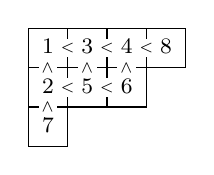
\begin{tikzpicture}
            \footnotesize
            \draw
                (0,0) -- (0,1.5) -- (2,1.5) -- (2,1) -- (1.5,1) -- (1.5,0.5) -- (0.5,0.5) -- (0.5,0) -- cycle
                (0,0.5) -- ++(0.5,0)
                (0,1) -- ++(1.5,0)
                (0.5,0.5) -- ++(0,1)
                (1,0.5) -- ++(0,1)
                (1.5,1) -- ++(0,0.5)
            ;
    
            \begin{scope}[text height=1.5ex,text depth=0.25ex]
                \begin{scope}[every node/.style={fill=white,inner sep=1.5pt}]
                    \tiny
                    \node at (0.5,1.25) {$<$};
                    \node at (1  ,1.25) {$<$};
                    \node at (1.5,1.25) {$<$};
                    \node at (0.5,0.75) {$<$};
                    \node at (1  ,0.75) {$<$};
        
                    \node [rotate=-90] at (0.25,1)   {$<$};
                    \node [rotate=-90] at (0.75,1)   {$<$};
                    \node [rotate=-90] at (1.25,1)   {$<$};
                    \node [rotate=-90] at (0.25,0.5) {$<$};
                \end{scope}
    
                \node at (0.25,0.25) {7};
                \node at (0.25,0.75) {2};
                \node at (0.25,1.25) {1};
                \node at (0.75,0.75) {5};
                \node at (0.75,1.25) {3};
                \node at (1.25,0.75) {6};
                \node at (1.25,1.25) {4};
                \node at (1.75,1.25) {8};
            \end{scope}
        \end{tikzpicture}
        \caption{Example standard Young tableau.}
        \label{fig:SYTex}
    \end{figure}
    \begin{itemize}
        \item We start with a Young diagram.
        \item We need to fill it with 8 numbers.
        \item There are relations between the boxes.
        \item Some constraints on what can go where, but there are more of them.
        \item So there are three $\SYT_8$. Call a tableaux within here $T$.
    \end{itemize}
    \item Theorem: $\dim V_\lambda$ is the number of SYTs of shape $\lambda$.
    \item Examples.
    \begin{figure}[h!]
        \centering
        \begin{subfigure}[b]{0.15\linewidth}
            \centering
            \begin{ytableau}
                1\\
                2\\
                3\\
                4\\
            \end{ytableau}
            \caption{$\Delta(1234)$.}
            \label{fig:SYT4a}
        \end{subfigure}\\[1em]
        \begin{subfigure}[b]{0.15\linewidth}
            \centering
            \begin{ytableau}
                1 & 3 & 4\\
                2\\
            \end{ytableau}
            \caption{$(x_1-x_2)$.}
            \label{fig:SYT4b}
        \end{subfigure}
        \begin{subfigure}[b]{0.15\linewidth}
            \centering
            \begin{ytableau}
                1 & 2 & 4\\
                3\\
            \end{ytableau}
            \caption{$(x_1-x_3)$.}
            \label{fig:SYT4c}
        \end{subfigure}
        \begin{subfigure}[b]{0.15\linewidth}
            \centering
            \begin{ytableau}
                1 & 2 & 3\\
                4\\
            \end{ytableau}
            \caption{$(x_1-x_4)$.}
            \label{fig:SYT4d}
        \end{subfigure}\\[1em]
        \begin{subfigure}[b]{0.23\linewidth}
            \centering
            \begin{ytableau}
                1 & 2\\
                3 & 4\\
            \end{ytableau}
            \caption{$(x_1-x_3)(x_2-x_4)$.}
            \label{fig:SYT4e}
        \end{subfigure}
        \begin{subfigure}[b]{0.23\linewidth}
            \centering
            \begin{ytableau}
                1 & 3\\
                2 & 4\\
            \end{ytableau}
            \caption{$(x_1-x_2)(x_3-x_4)$.}
            \label{fig:SYT4f}
        \end{subfigure}
        \caption{Standard Young tableaux of 4.}
        \label{fig:SYT4}
    \end{figure}
    \begin{enumerate}
        \item Only ONE way to fill trivial and alternating Young diagrams.
        \item Three ways to fill $(3,1)$.
        \item Two ways to fill $(2,2)$.
    \end{enumerate}
    \item Learn the representations of $S_4$ by heart!
    \item Proving the theorem.
    \begin{proof}
        How are these tableaux related to the basis of $\Sp_\lambda$?

        For a SYT, consider the polynomial $\Sp(T)$ (take a particular filling and write down the polynomials; \emph{see how to do so by the corresponding polynomials next to examples above in picture}.).

        Notice that the $\Sp(T)$ form a basis of $V_{\lambda'}$. From here on out, the proof is quite subtle.

        Obvious part of the proof: Lemma: $S_n,\lambda$ fixed implies that the $\Sp(T)$, where $T\in\SYT_\lambda$ (i.e., $T$ is a SYT of shape $\lambda$), are linearly independent. They are each linearly independent because each contains a certain monomial that none of the others contain; specifically, this will be the lexicographically smallest monomial $SM$.
        \begin{proof}
            Consider the lexicographically smallest monomial in $\Sp(T)$ (the Specht polynomial of tableau $T$). Our goal is to reconstruct $T$ from it.

            Example of how to do this: Note: We have the same lemma as last time: $SM(PQ)=SM(P)SM(Q)$. Starting from the example on the previous blackboard, we have $\Delta(x_1,x_2,x_7)$. Smallest monomial is $x_2x_7^2x_5x_6$. This follows from the determinant interpretation of the vandermonde determinant polynomials by looking at all the smallest combinations we can put together, which goes along the diagonal of the matrix, e.g., $1\cdot x_2\cdot x_7^2$. From this monomial, we can reconstruct the SYT by putting $x_7$ in the bottom by necessity, then we have to put $2,5,6$ (other coefficients of SM) above in the certain order to get the right ordering. Then, we have to put the ones that aren't there ($x_1^0x_3^0x_4^0x_8^0)$ in the top row. This gives us our YT back.
            
            We will not give a rigorous proof here; the above example is illustrative.
        \end{proof}
        Rudenko will not finish this one.
    \end{proof}
    \item Corollary: $\dim V_\lambda=\dim V_{\lambda'}$.
    \begin{proof}
        Any representation of $S_n$ will be self-dual.
    \end{proof}
    \item Fact: We have the following identity.
    \begin{equation*}
        V_{\lambda'} = V_\lambda\otimes(\text{sign})
    \end{equation*}
    \item Let $f_\lambda$ be the number of SYTs of shape $\lambda$. We have shown that $f_\lambda\leq\dim(V_\lambda)$.
    \item Theorem (RSK): There exists a bijection between permutations in $S_n$ and pairs of SYTs of the same shape (i.e., of \textbf{area} $n$).
    \begin{itemize}
        \item RSK stands for Robinson-Schensted-Knuth.
    \end{itemize}
    \item Corollary: $f_\lambda=\dim V_\lambda$.
    \begin{proof}
        $\sum_{\lambda=\text{YT of area }n}f_\lambda^2
        = n!
        = \sum(\dim V_\lambda^2)$.
        This is enough to prove that $f_\lambda\leq\dim V_\lambda$ and $f_\lambda=\dim V_\lambda$.
    \end{proof}
    \item Let's see how this stuff works through an example.
    \begin{itemize}
        \item Let's take permutation
        \begin{equation*}
            \sigma = (13)(27654) =
            \begin{pmatrix}
                1 & 2 & 3 & 4 & 5 & 6 & 7 & 8\\
                3 & 7 & 1 & 2 & 4 & 5 & 6 & 8\\
            \end{pmatrix}
            \in S_8
        \end{equation*}
        \item Start with a pair of YTs.
        \item Start with the number written first (3) and then put 1. You take the empty tableaux and insert $[3]$ inside.
        \item We now have a new pair of tableaux. How do we insert the next number (7)? Try adding it to the right, then add 2 to the right of the second one in correspondence.
        \item How do we insert the next number (1)? Push out 3 with 1 and move 3 to the next row. In the second one, there's one new square in the bottom position, so we add it there.
        \item Next number: 2 pushes out 7. Four goes in the new box. 
        \item 4 gets inserted to the right; 5 fills the new box.
        \item 5,6,8 go further to the right; 6,7,8 in the second one.
        \item Now we have a pair of tableaux.
        \item This is an algorithm that, for every permutation, gives us a pair of tableaux.
    \end{itemize}
    \item Why does this work?
    \begin{itemize}
        \item Everything is increasing in rows.
        \item If $y>x$, we need to insert it in the row below but to the left.
        \item Perhaps its starting with $y$ in the top row and then it being displaced down and to the left by $x$.
        \item Every time we add something bigger, we add a corner box.
        \item This algorithnm proves the theorem.
        \item I really need to think about this!!
    \end{itemize}
    \item This algorithm takes us between a pair $(T,T')$ of young tableaux to a permutation $\sigma$.
    \item Many interesting properties that are hard to prove. Here's a few.
    \begin{enumerate}
        \item The map takes $(T',T)\mapsto\sigma^{-1}$.
    \end{enumerate}
    \item $\lambda_1$ and $\lambda_1'$ are the length of the longest increasing (resp. decreasing) subsequence of your permutation variables.
    \item Last word: There is a famous theorem called the \textbf{Erd\H{o}s-Szekeres theorem}.
    \item This correspondence is a deep way to understand permutations/sequences of numbers. This is a big tool in CS.
    \item Next time: Induction restriction.
\end{itemize}




\end{document}